% mnras_template.tex
%
% LaTeX template for creating an MNRAS paper
%
% v3.0 released 14 May 2015
% (version numbers match those of mnras.cls)
%
% Copyright (C) Royal Astronomical Society 2015
% Authors:
% Keith T. Smith (Royal Astronomical Society)

% Change log
%
% v3.0 May 2015
%    Renamed to match the new package name
%    Version number matches mnras.cls
%    A few minor tweaks to wording
% v1.0 September 2013
%    Beta testing only - never publicly released
%    First version: a simple (ish) template for creating an MNRAS paper

%%%%%%%%%%%%%%%%%%%%%%%%%%%%%%%%%%%%%%%%%%%%%%%%%%
% Basic setup. Most papers should leave these options alone.
\documentclass[a4paper,fleqn,usenatbib]{mnras}

% MNRAS is set in Times font. If you don't have this installed (most LaTeX
% installations will be fine) or prefer the old Computer Modern fonts, comment
% out the following line
\usepackage{newtxtext,newtxmath}
% Depending on your LaTeX fonts installation, you might get better results with one of these:
%\usepackage{mathptmx}
%\usepackage{txfonts}

% Use vector fonts, so it zooms properly in on-screen viewing software
% Don't change these lines unless you know what you are doing
\usepackage[T1]{fontenc}
\usepackage{ae,aecompl}

%%%%% AUTHORS - PLACE YOUR OWN PACKAGES HERE %%%%%

% Only include extra packages if you really need them. Common packages are:
\usepackage{graphicx}	% Including figure files
\usepackage{amsmath}	% Advanced maths commands
\usepackage{amssymb}	% Extra maths symbols
\usepackage[xindy]{glossaries}

%%%%%%%%%%%%%%%%%%%%%%%%%%%%%%%%%%%%%%%%%%%%%%%%%%

%%%%% AUTHORS - PLACE YOUR OWN COMMANDS HERE %%%%%

% Please keep new commands to a minimum, and use \newcommand not \def to avoid
% overwriting existing commands. Example:
%\newcommand{\pcm}{\,cm$^{-2}$}	% per cm-squared

\newcommand{\GSF}[1]{\noindent\textcolor{blue}{GSF:#1}}

\makeglossaries

%glossary
\newacronym{alfa}{ALFA}{Arecibo L-Band Feed Array}
\newacronym{dm}{DM}{Dispersion Measure}
\newacronym{frb}{FRB}{Fast Radio Burst}
\newacronym{fwhm}{FWHM}{Full-Width at Half-Maximum}
\newacronym{gbt}{GBT}{Greenbank Telescope}
\newacronym{igm}{IGM}{Intergalactic Medium}
\newacronym{ism}{ISM}{Interstellar Medium}
\newacronym{nip}{NIP}{Non-image Processing}
\newacronym{rfi}{RFI}{Radio-frequency Interference}
\newacronym{ska}{SKA}{Square Kilometre Array}
\newacronym{sefd}{SEFD}{System Equivalent Flux Density}
\newacronym{snr}{SNR}{Signal-to-Noise Ratio}
\newacronym{sps}{SPS}{Single Pulse Search}

%%%%%%%%%%%%%%%%%%%%%%%%%%%%%%%%%%%%%%%%%%%%%%%%%%

\title[ALFABURST Initial]{ALFABURST Initial}

\author[ALFABURST Team]{
ALFABURST Team
}

% These dates will be filled out by the publisher
\date{Accepted XXX. Received YYY; in original form ZZZ}

% Enter the current year, for the copyright statements etc.
\pubyear{2017}

% Don't change these lines
\begin{document}
\label{firstpage}
\pagerange{\pageref{firstpage}--\pageref{lastpage}}
\maketitle

% Abstract of the paper
\begin{abstract}
% What is the point of the paper?
% What is the context of the study? What background information is necessary to understand the study?
% How was the study done?
% What is the main take away message?
% What can be said about these results, and how does this affect future work?
The ALFABURST fast radio burst (FRB) survey has been observing commensally with
other projects using the ALFA receiver since July 2015. We report on the
non-detection of any FRBs from that time until May 2017. With current FRB rate
models we expected to see multiple FRBs in based on the total observing time,
telescope sensitivity and beam size. We discuss the implications for this
non-detection FRBs in the context of recent detections with other telescopes.
\end{abstract}

% Select between one and six entries from the list of approved keywords.
% Don't make up new ones.
\begin{keywords}
radio continuum: transients -- methods: observational
\end{keywords}

%%%%%%%%%%%%%%%%%%%%%%%%%%%%%%%%%%%%%%%%%%%%%%%%%%

%%%% TO REVIEW
% 0709.4301 (First FRB) [Jayanth]
% 1109.2659 (Bright FRB rates with ATA) [Jayanth]
% 1307.1200 (FRB Standard Candle Model) [Griffin]
% 1307.1628 (4 FRBs from HTRU and sky rates) [Golnoosh]
% Madau & Dickinson 2014 (Star Formation Rate Review) [Griffin]
% 1404.2934 (Repeater FRB) [Kaustubh]
% 1412.0342 (HTRU FRB) [Golnoosh]
% 1505.05893 (Scintillation Effects of FRB Sky Distribution) [Griffin]
% 1601.03547 (FRBCAT) [Golnoosh]
% 1603.08880 (Repeater Additional Bursts) [Kaustubh]
% Champion et al 2016 (5 FRBs from HTRU) [Golnoosh]
% Caleb et al 2016 (UTMOST Initial Survey) [Mayuresh]
% 1611.05758 (Bright Parkes FRB) [Mayuresh]
% Chatterjee et al 2017 (Repeater VLA Localization) [Kaustubh]
% 1701.01099 (Repeater EVN Localization) [Kaustubh]
% 1701.01100 (Repeater Redshift and Host) [Kaustubh]
% 1702.08040 (Initial CHIME Survey) [Mayuresh]
% 1703.10173 (3 FRBs from UTMOST) [Golnoosh]
% 1705.07553 (Repeater Multi- radio-freq observations) [Kaustubh]
% 1705.07581 (ASKAP First Bright FRB) [Golnoosh]
% 1705.07698 (Repeater Star Forming Region) [Kaustubh]

\section{Introduction}

\section{ALFABURST Overview}

ALFABURST is an \gls*{frb} search instrument which has been used to commensally
observe since July 2015 with other \gls*{alfa} observations at Arecibo
Observatory. This system is a component of the SETIBURST back-end
\citep{2017ApJS..228...21C} and uses ARTEMIS \citep{2015MNRAS.452.1254K} for
automated, real-time detection. During this time period an \gls*{sps} was
performed from \gls*{dm} 0 to 10000, pulse width from $256 \mu s$ to $16$ ms,
across a 56 MHz bandwidth for all 7 beams. Detection above an \gls*{snr} of 10
were recorded along with an $8.4$ second dynamic spectrum window around the
event. If multiple events were detected in the same time window, these events
were pooled together.  Approximately 150k windows were recorded between July
2015 and June 2017, the vast majority of which are false detections due to
\gls*{rfi} signals passing through the real-time \gls*{rfi} exciser. We detect
no \glspl*{frb} in our commensal survey.

A wide-feature, learned model was used to classify the event windows in order to
filter out \gls*{rfi} and create a priority queue for visual examination. This
model and the post-processing procedures are discussed in Section
\ref{sec:event_classify}. We discuss the expected event rates in Section
\ref{sec:frb_rates} and consider possible explanations for our non-detection
result in Section \ref{sec:discuss}.

%%% OBSERVATION TIME BEGINS %%%

From the beginning of July 2015 to the end of May 2017 \gls*{alfa} has been
used for approximately 1400 hours of observing, with all seven beams
functional. Due to pipeline development and hardware reliability ALFABURST was
active and functional for on average 350 hours per beam.  The current system is
setup to be reliably in use for all beams any time \gls*{alfa} is active and in
the correct receiver turret position. Of the survey coverage, approximately
65\% of the time has been in pointings out of the galactic plane ($|b| >
5^{\circ}$). Since we are searching up to a \gls{dm} of 10000 the survey is
still sensitive to \glspl{frb} at cosmological distances when observing in the
galactic plane. But, scintillation effects can reduce the overall \gls{frb}
event rates \citep{2015MNRAS.451.3278M}.

%%% OBSERVATION TIME ENDS   %%%

%%% SENSITIVITY BEGINS %%%
\subsection{FRB Survey Metric}
\label{sec:survey_metric}

Using the survey observing time and the \gls{alfa} beam size we can derive the
\gls{frb} survey metric of square-degree hours. An \gls*{alfa} beam is
approximately 3.8' x 3.3' at \gls*{fwhm} across the band.  Using this beam size
and the average observation time per beam the telescope-independent \gls*{frb}
survey coverage metric for ALFABURST as of June 2017 is 6.7 square-degree hours.
This is a fairly small survey metric becuase of the small beam size. But, we are
only taking into account the beam size out to the \gls{fwhm}. We can take into
acount the entire first sidelobes of the beams as Arecibo would be senstive
enough to detect most previous \glspl{frb} in the first sidelobes. Using the
parameterized \gls{alfa} beam model (Figure \ref{fig:alfa_beam})
\citep{GALFAbeam} we can compute the \gls{frb} survey metric as a function of
the minimum \gls{alfa} sensitvity (Figure \ref{fig:survey_metric}).

% alfaburst-initial-survey/notebooks/ALFA_Beam_Response.ipynb
\begin{figure}
    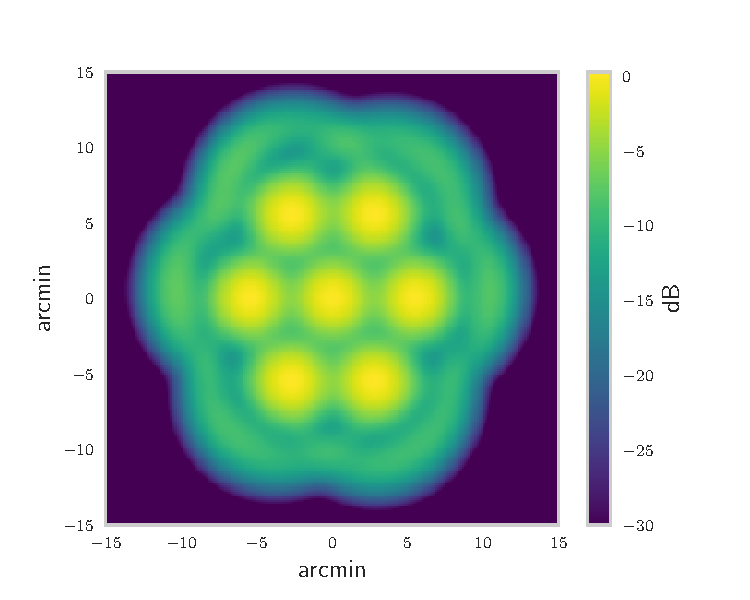
\includegraphics[width=1.0\linewidth]{figures/ALFA_beam_1425MHz_dB.pdf}
    \caption{Primary lobe and first sidelobe model of the AFLA receiver in
    decibels. The sidelobes are sensitive many of the previously detected FRBs.
    }
    \label{fig:alfa_beam}
\end{figure}

% alfaburst-initial-survey/notebooks/ALFA_Beam_Response.ipynb
\begin{figure}
    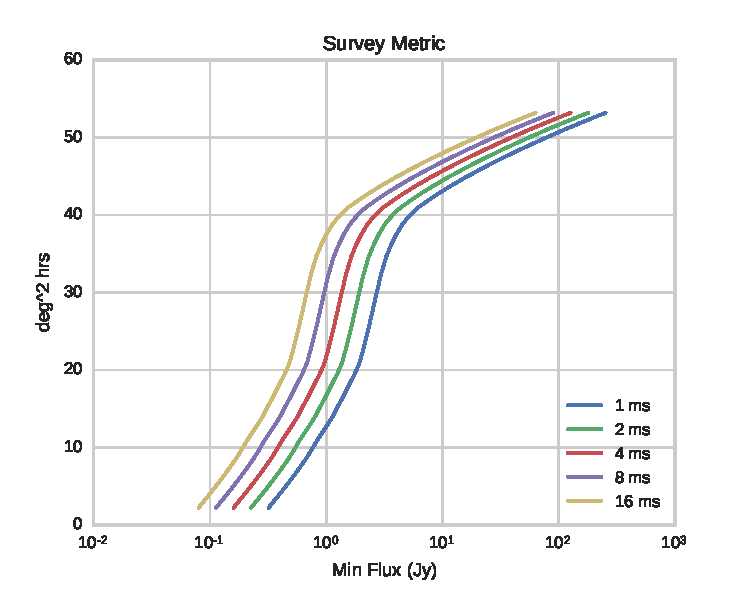
\includegraphics[width=1.0\linewidth]{figures/survey_metric.pdf}
    \caption{ALFABURST FRB survey metric for pulses of different widths,
    accounting for the ALFA primary beam and first sidelobe sensitivity.
    }
    \label{fig:survey_metric}
\end{figure}

% TODO: relate beam gain to sensitivity
% TODO: relate this figure to previously detected FRBs
% TODO: how does this metric compare to other surveys?
% TODO: how does this compare to expected rates?
% TODO: why is ALFABURST useful? sensitivity

Using Equation 6 of \cite{2015MNRAS.452.1254K}, a \gls*{sps} pipeline is
sensitive to pulses with a minimum flux density (in Jy) of
%
\begin{equation}
S_{min} = \textrm{SEFD} \frac{\textrm{SNR}_{min}}{\sqrt{D \; \Delta \tau \;
\Delta \nu}}
\end{equation}
%
which is a function of the telescope \gls*{sefd}, the minimum \gls*{snr}
detection level $\textrm{SNR}_{min}$ and the decimation rate $D$ compared to the
native instrumental time resolution $\tau$, this comes from the search pipeline
which averages together spectra to search for scattered pulses. ALFABURST has a
native resolution of $\Delta \tau = 256 \; \mu s$, effective bandwidth $\Delta
\nu = 56 \textrm{MHz}$, and $\textrm{SNR}_{min} = 10$. The \gls*{sefd} of the
\gls*{alfa} receiver is approximately 3 Jy across the band for all beams.

%%% SENSITIVITY ENDS   %%%

%%% SKY COVERAGE BEGINS %%%

Since ALFABURST was installed, the majority of ALFA observation time is
allocated for the AGES \citep{2006MNRAS.371.1617A} and PALFA
\citep{2006ApJ...637..446C} surveys (Figure \ref{fig:sky_coverage}).  The AGES
survey pointing is off the galactic plane, thus there is little dispersion and
scattering due to the galactic \gls*{ism}. PALFA is a pulsar search survey with
pointings near the galactic plane. These lines of sight can introduce
significant dispersion due to the \gls*{ism}. We search out to a DM of 10000
which is well beyond the maximum galactic dispersion, even when \gls*{igm}
dispersion is accounted for from sources of cosmological distances.

% alfaburst-initial-survey/notebooks/Sky_Coverage.ipynb
\begin{figure*}
    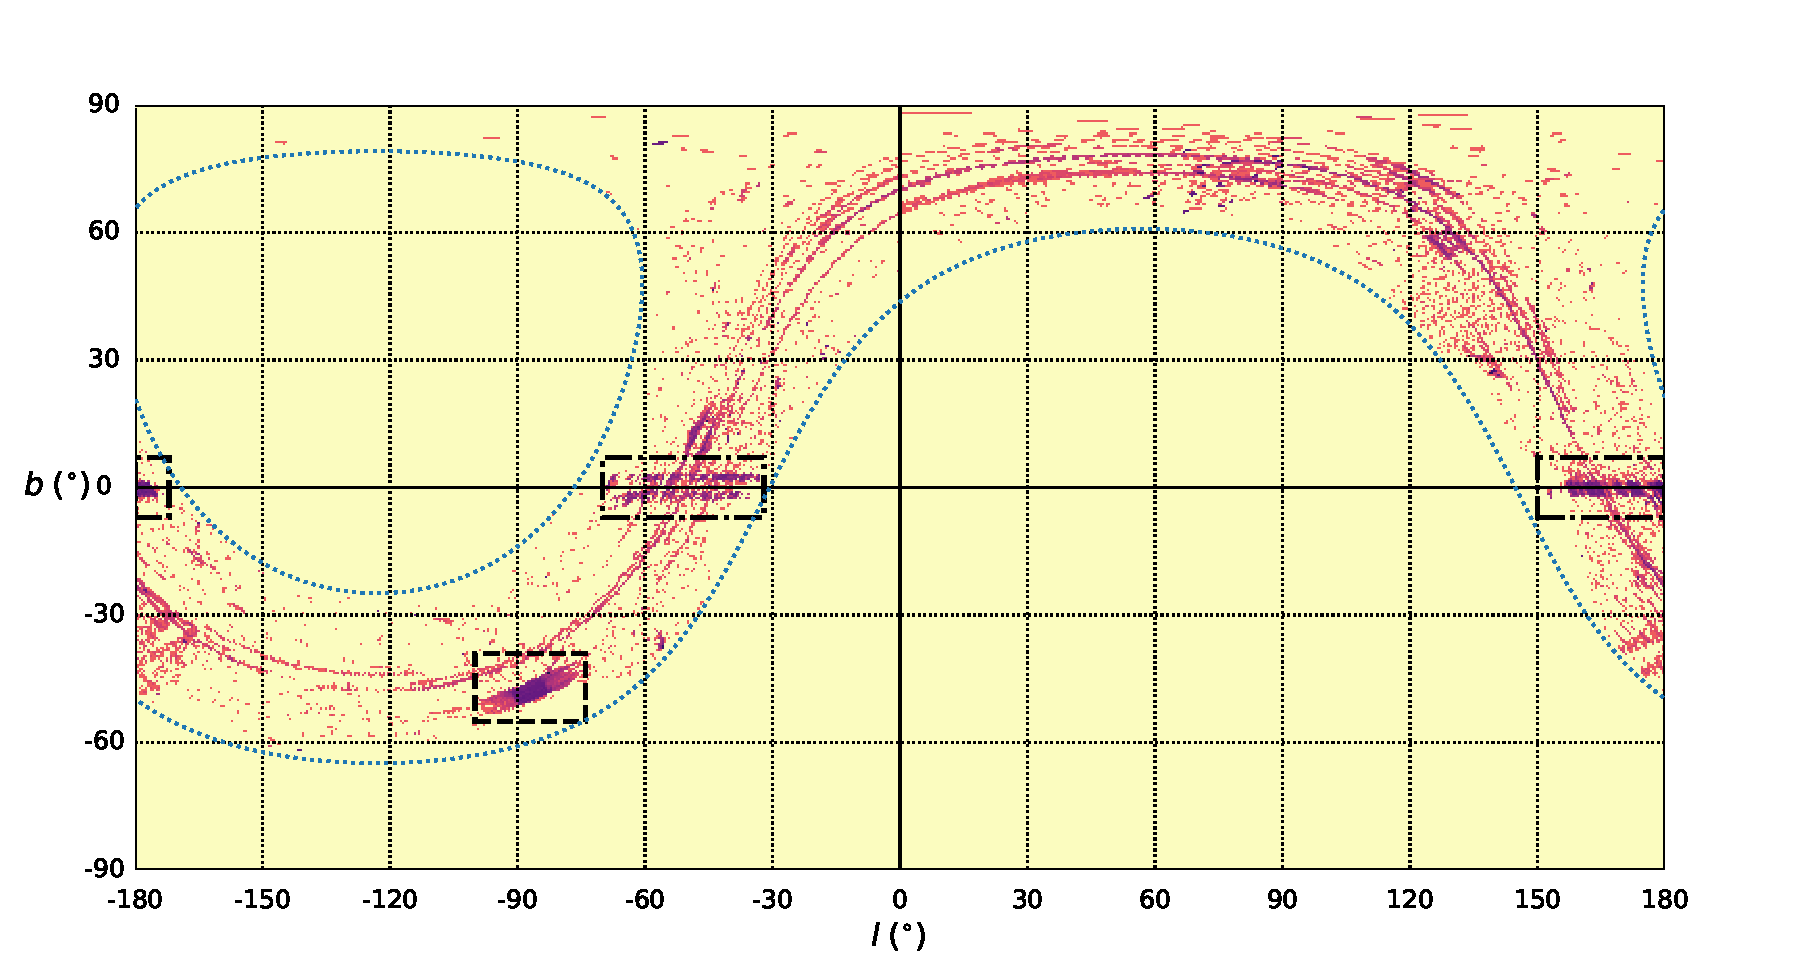
\includegraphics[width=1.0\linewidth]{figures/cartview_sky_coverage.pdf}
    \caption{Sky coverage during ALFA usage between July 2015 and June 2017,
    shown in a Cartesian projection in galactic coordinates. Color represents
    total time pointing in a log scale. The majority of ALFA usage during this
    time was for the PALFA survey along the galactic plane (dot-dashed boxes)
    and the AGES survey (dashed box).  The S-shaped arcs across the plot are due
    to fixed pointings in local azimuth and altitude.
    }
    \label{fig:sky_coverage}
\end{figure*}

%%% SKY COVERAGE ENDS   %%%

%%% SYSTEM VERIFICATION BEGINS %%%

PALFA scheduling regularly observe known pulsars to verify timing analysis,
this provides a consistent verification of our \gls*{sps} to detect
pulses. As the PALFA survey is performed in the galactic plane a number of high
\gls*{dm} pulsars were observed, single pulses from B1859+03 (\gls*{dm}: 402),
B1900+01 (\gls*{dm}: 245), B2002+32 (\gls*{dm}: 234), B1933+16 (\gls*{dm}: 158),
among others were detected.

% TODO: figure: B1900+01 pulse (dynamic spectrum, intergrated dedispered time
% series)

%%% SYSTEM VERIFICATION ENDS   %%%

\section{Event Prioritization and Classification}
\label{sec:event_classify}

% Event Classification and Prioritization
%   * priority classifier model
%       * labelled data
%       * wide feature selection + classifier
%       * deep feature selection + classifier
%   * event statistics

\section{Implied Low-Flux FRB Rates}
\label{sec:frb_rates}

% Low flux FRB limits from ALFABURST
%   * survey coverage compare: HTRU/Parkes, ASKAP, GBT, ATA, Molongolo
%   * update to standard candle model using the repeater
%   * log n - log s curve
%   * expected rates based on non-detection, observation time, and FRB standard
%   candle model, use fluence
%   * Do we expect to see the known frbs at a further distance which we are probing?

% Bright FRB rates:
%   * calcutlate beam size (including sidelobes) which is sensitive to bright
%   FRBs. Cordes et al 2006 and Spitler et al 2014 present an ALFA beam model

\section{Discussion}
\label{sec:discuss}

% Possible reasons: star formation rate, scintillation, steep spectrum
%   * Star formation rate:
%       * implied FRB Luminosity function: cosmological star formation rate, peaks
%       around z=2? write notebook to produce rates, Madau & Dickinson 2014
%   * scintillation:
%       * limited bandwidth, repeater band varys
%       * relation to Macquart and Johnston paper: rate off/on the plane is
%       different due to scintillation regimes
%       * repeater and low freq frb searches: spectra are not pulsar like. may be
%       due to strong scintillation
%   * steep spectrum/band limited:
%       * relation to ASKAP detections
%       * Law et al see no detections at low and 5 GHz+ freqs -> band limited,
%       steep spectrum

\section{Future Work}
\label{sec:future_work}

The current \gls*{sps} pipeline is undergoing a significant upgrade. The input
bandwidth is limited to 56 MHz of the full 336 MHz digital band due to IO
limitations. A new pipeline developed for \gls*{ska} \gls*{nip} will be used to
process the full \gls*{alfa} band. This will increase sensitivity, and improve
detection rate if \glspl*{frb} scintillate similar to FRB121102. An improved
version of the real-time \gls*{rfi} exciser is currently being developed and
will be deployed to reduce the false detection rate. The post-processing
classifier and prioritizer model is being updated to make use of an auto-encoder
to select deep features and auto-generate classes.

Over the time period ALFABURST has been active, the use of \gls*{alfa} has
decreased as the PALFA and AGES surveys end. The 327 MHz and L-band wide feeds
are commonly used. We are generalizing the \gls*{alfa} specific \gls*{sps}
pipeline to be used when these feeds are active, increasing our survey time and
sampling a larger portion of frequency space. Additionally, our search pipeline
will be duplicated for use on the \gls*{gbt} to be commensally run with L-band
observations. 

\bibliographystyle{mnras}
\bibliography{alfaburst.bib} 

\bsp	% typesetting comment
\label{lastpage}
\end{document}

% End of mnras_template.tex
